% !TEX TS-program = xelatex
% !TEX encoding = UTF-8 Unicode
% !TEX spellcheck = de_DE
% 
% © 2016 Moritz Brinkmann, CC-by-sa
% http://latexkurs.github.io

\documentclass[
	vorläufig=false, 
	blattnr=6,
	ausgabe=2016-12-02,
	abgabe=2016-12-09,
	lösung,
	shortverb,
]{../tex/latexkurs-exercise}

\usepackage{mathtools, siunitx, booktabs, pgfplots}


\begin{document}


\begin{aufgabe}[6]{Daten darstellen mit pgfplots}
	Bei einer Umfrage sind die in Tabelle \ref{tab:umfrage} dargestellten Daten erhoben worden.
	Diese Daten sollen Sie jetzt grafisch aufbereiten. 
	\begin{table}[h]
		\newcommand{\rth}[1]{\rotatebox{50}{\textsf{{#1}}}}
		\centering
		\begin{tabular}{l*{5}{S[table-number-alignment=left]}}
%			\toprule
			\textsf{{Frage}} & \rth{furchtbar} & \rth{meh} & \rth{ganz gut} & \rth{genial} & \rth{keine Ang.} \\
			\toprule
			Wie finden Sie Himbeereis? & 9 & 1 & 2 & 186 & 0 \\
			Mögen Sie Tanzen? & 32 & 63 & 52 & 49 & 2 \\
			Was halten Sie von Topf\/pflanzen? & 28 & 17 & 12 & 26 & 115 \\
			\bottomrule
		\end{tabular}
		\caption{Umfrage\/ergebnisse}
		\label{tab:umfrage}
	\end{table}
	\noindent Nutzen Sie das Paket \pkg{pgfplots} um die Ergebnisse darzustellen. 
	Lassen Sie sich ruhig von der Paketdokumentation inspirieren und wählen Sie den Diagrammtyp oder die
	Diagrammtypen, die Sie für besonders geeignet halten. Je nach Darstellung können Sie dabei alle Daten in
	ein Diagramm eintragen, oder für jede Frage ein eigenes Diagramm erstellen.
	\abgabe{Quellcode per Mail{,} Quellcode und fertiges Dokument ausgedruckt.}
\end{aufgabe}

\lösung{06_loesung_umfrage}

\vskip2em

\noindent Von den folgenden beiden Aufgaben müssen Sie nur eine bearbeiten! Die erste richtet sich vor allem an Mathematiker*innen, die zweite eher an Physiker*innen. Welche genau Sie bearbeiten steht Ihnen selbstverständlich frei. Sie können nur für eine Aufgabe Punkte erhalten, dafür gibt es aber bis zu sechs Bonuspunkte.

\begin{aufgabe}[6]<6>{Schlangenlemma (Aufgabe für Mathematiker*innen)}
	Das Schlangenlemma\footnote{Wer nichts mit dem Begriff anfangen kann wird auf
	\href{https://de.wikipedia.org/wiki/Schlangenlemma}{Wikipedia} oder im 
	\href{https://books.google.com/books?id=Fge-BwqhqIYC&pg=PA157}{Algebra-Buch} des Vertrauens fündig.}
	ist ein wichtiges Werkzeug in der homologischen Algebra, für das man kommutative Diagramme benutzt.
	Das in Abbildung \ref{fig:snake1} gezeigte Diagram wird im Schlangenlemma zum sogenannten 
	Schlangendiagramm (Abbildung \ref{fig:snake2}) erweitert.

	\begin{figure}[h]
		\centering
		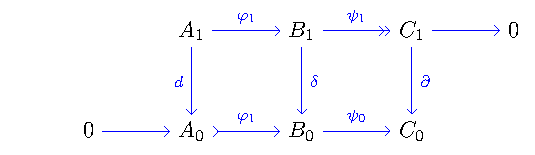
\includegraphics{06_snake1}
	  \caption{kommutatives Diagramm mit exakten Zeilen}
	  \label{fig:snake1}
	\end{figure}
	
	\begin{figure}[h]
		\centering
		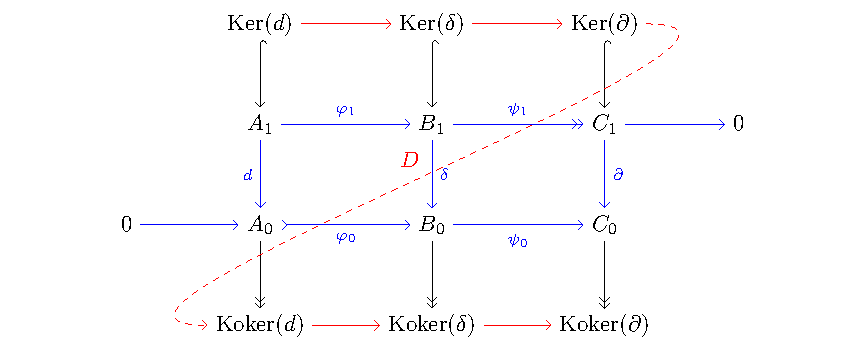
\includegraphics{06_snake2}
		\caption{Schlangendiagramm (Das Schlangenlemma hat seinen Namen vom Pfeil $D$, der sich wie eine
			Schlange durch das Diagramm windet)}
		\label{fig:snake2}
	\end{figure}

	\noindent Da jede Mathematiker*in wissen sollte, wie man kommutative Diagramme \TeX t soll das hier 
	anhand des Schlangendiagramms geübt werden.
	\begin{enumerate}[label=\alph*)]
		\item Reproduzieren Sie das in Abbildung \ref{fig:snake2} gezeigte Diagramm in \LaTeX. Sie müssen
		sich dabei nicht an die hier verwendeten Pfeile und Farben, oder die Notation halten. Inhaltlich 
		sollen sich die Diagramme aber entsprechen. Achten Sie darauf, dass mathematische Ausdrücke auch 
		innerhalb der Abbildung im Mathemodus gesetzt werden.
		
		 Es gibt diverse Pakete, die Ihnen dabei die Arbeit erleichtern können. So lassen sich kommutative 
		 Diagramme zum Beispiel relativ elegant mit \TikZ\footnote{Hierfür eignet sich besonders die
		 |matrix|-Library.} erzeugen.
		
		\item \emph{Bonusaufgabe:} Setzen Sie das komplette Schlangenlemma inklusive Beweis.
		%Sie können den Text dabei ruhig aus der e-Version eines Mathebuchs kopieren.
		
		Nutzen Sie dafür die \hologo{AmS}-Pakete und definieren Sie sich die nötigen Operatoren und 
		Umgebungen mit |\DeclareMathOperator| und |\newtheorem| selbst. Die 
		Darstellung der mathematischen Elemente im Text und in den Abbildungen (Diagrammen) sollen 
		selbstverständlich gleich sein. 
	\end{enumerate}
	\abgabe{Quellcode per Mail{,} Quellcode und fertiges Dokument ausgedruckt.}
\end{aufgabe}

\lösung{06_loesung_schlangenlemma}


\begin{aufgabe}[6]<6>{Zerfallsprozess (Aufgabe für Physiker*innen)}
	Sie haben den Zerfall eines Radioaktiven Isotops gemessen und müssen das Ergebnis nun 
	grafisch darstellen. 
	\begin{enumerate}[label=\alph*)]
		\item Laden Sie sich die Datei 
		\href{http://latexkurs.github.io/exercises/06_messwerte.dat}{\texttt{06\_messwerte.dat}} von der
		Vorlesungshomepage herunter und stellen Sie die darin enthaltenen Daten mithilfe des Pakets
		\pkg{pgfplots} dar. Ordnen Sie dabei die Spalten wie folgt zu und stellen Sie sicher, dass auch der
		Messfehler im Diagramm zu sehen ist.
		\begin{center}
			\begin{tabular}{rl}
				\toprule
				\textbf{Spalte} & \textbf{Zuordnung}\\
				\midrule
				|zeit| & |x| \\
				|zerfaelle| & |y| \\
				|zerfaelle_err| & |y error|\\
				\bottomrule
			\end{tabular}
		\end{center}
		\item \emph{Bonusaufgabe:} Nutzen Sie \LaTeX\ um die Zerfallskonstante $\lambda$ zu berechnen und
		zeichnen Sie die theoretische Kurve in das Diagramm zu den Messwerten. Welche Darstellung ist
		besonders geeignet um die mathematische Natur des Zerfallsgesetzes zu demonstrieren?
	\end{enumerate}
	\abgabe{Quellcode per Mail{,} Quellcode und fertiges Dokument ausgedruckt.}
\end{aufgabe}

\lösung{06_loesung_zerfall}

\end{document}